\documentclass[utf8x, 12pt]{G7-32} 
\sloppy

% Настройки стиля ГОСТ 7-32
% Для начала определяем, хотим мы или нет, чтобы рисунки и таблицы нумеровались в пределах раздела, или нам нужна сквозная нумерация.

%\EqInChapter % формулы будут нумероваться в пределах раздела
%\TableInChapter % таблицы будут нумероваться в пределах раздела
%\PicInChapter % рисунки будут нумероваться в пределах раздела

% Добавляем гипертекстовое оглавление в PDF
\usepackage[
bookmarks=true, colorlinks=true, unicode=true,
urlcolor=black,linkcolor=black, anchorcolor=black,
citecolor=black, menucolor=black, filecolor=black,
]{hyperref}

% Изменение начертания шрифта --- после чего выглядит таймсоподобно.
% apt-get install scalable-cyrfonts-tex

\IfFileExists{cyrtimes.sty}
    {
        \usepackage{cyrtimespatched}
    }
    {
        % А если Times нету, то будет CM...
    }

\usepackage{graphicx}   % Пакет для включения рисунков
\DeclareGraphicsExtensions{.jpg,.pdf,.png}
% С такими оно полями оно работает по-умолчанию:
% \RequirePackage[left=20mm,right=10mm,top=20mm,bottom=20mm,headsep=0pt]{geometry}
% Если вас тошнит от поля в 10мм --- увеличивайте до 20-ти, ну и про переплёт не забывайте:
\geometry{right=20mm}
\geometry{left=30mm}



% Произвольная нумерация списков.
\usepackage{enumerate}

\setcounter{tocdepth}{3} %Подробность оглавления
%4 это chapter, section, subsection, subsubsection и paragraph
%3 это chapter, section, subsection и subsubsection
%2 это chapter, section, и subsection
%1 это chapter и section
%0 это chapter.



\begin{document}

\frontmatter 
\begin{center} 

\large САНКТ-ПЕТЕРБУРГСИЙ ГОСУДАРСТВЕННЫЙ ПОЛИТЕХНИЧЕСКИЙ УНИВЕРСИТЕТ

\large Кафедра Компьютерных Систем и Программных Технологий \\[5.5cm] 

\huge ОТЧЕТ \\[0.6cm] % название работы, затем отступ 0,6см
\large по индивидуальному заданию\\
\large Дисциплина: <<Программное обеспечение распределенных вычислительных систем>>\\[3.7cm]

\end{center} 

\begin{flushright}
Выполнил: студент гр. 63501/2 \\
Пономарев М.A \\[1.2cm]


Преподаватель \\
Стручков И.В.
\end{flushright}


\vfill 

\begin{center} 
\large Санкт-Петербург \\
2015
\end{center} 

\thispagestyle{empty}

\thispagestyle{empty}
\setcounter{page}{0}
\tableofcontents
\clearpage
\mainmatter



\chapter{Задание (Вариант №7)}

Система учета успеваемости студентов. Операции удаленного объекта: добавить оценку за экзамен, получить средний балл по студенту, удалить записи о студентах со средним баллом < X. 

Сериализуемый объект: результат экзамена (имя студента, оценка).



\chapter{Выполнение}

\section{Диаграмма классов UML}



\section{Варианты использования}


\underline{Участник: преподаватель, студент, администратор}

Вариант использования: вход в систему

\begin{enumerate}
	\item Пользователь вводит логин и пароль
	\item Система проверяет наличие логин и соответствия с ним пароля
	\item Если проверка:
	\begin{itemize}
		\item успешна: Система авторизирует пользователя
		\item не успешна: Система выдает пользователю соответствующее сообщение
	\end{itemize}
	
\end{enumerate}

\bigskip

\underline{Участник: студент}

Вариант использования: получение информации об оценке по посещенному экзамену:

\begin{enumerate}
	\item Студент входит в Систему.
	\item Студент вводит год, курс, название предмета.
	\item Система проверяет наличие События со связью предмет--студент.
	\item Если событие:
	\begin{itemize}
		\item найдено: Система выдает оценку по экзамену
		\item не найдено: Система выдает студенту соответствующее сообщение
	\end{itemize}
	
\end{enumerate}


\bigskip


\underline{Участник: преподаватель}

Вариант использования: получение средней оценки по всем студентам по определенному экзамену

\begin{enumerate}
	\item Преподаватель входит в Систему.
	\item Преподаватель вводит год, курс, название предмета.
	\item Система проверяет есть ли события связанные с экзаменом.
	\item Система проверяет связан ли преподаватель с данным экзаменом
	\item Если обе проверки:
	\begin{itemize}
		\item успешны: Система выдает средний балл по экзамену
		\item не успешны: Система выдает преподавателю соответствующее сообщение
	\end{itemize}
	
\end{enumerate}


\newpage

\underline{Участник: администратор}

Вариант использования: Добавление преподавателя в базу данных

\begin{enumerate}
	\item Администратор входит в Систему.
	\item Администратор вводит необходимые данные для внесения преподавателя в базу.
	\item Система проверяет существует ли преподаватель со схожими данными.
	\item Если проверка:
	\begin{itemize}
		\item успешна: Система вносит преподавателя в базу
		\item не успешна: Система выдает администратору соответствующее сообщение
	\end{itemize}	
\end{enumerate}

\bigskip

\underline{Участник: администратор}
  
Вариант использования: Изменение оценки по экзамену на определенную дату

\begin{enumerate}
	\item Администратор входит в Систему.
	\item Администратор вводит год, курс, название предмета, дату проведенного экзамена и оценку
	\item Система проверяет существует ли Событие по внесенной информации
	\item Система проверяет различны ли изменяемая и прошлая оценки
	\item Если обе проверки:
	\begin{itemize}
		\item успешны: Система изменяет оценку по экзамену
		\item не успешны: Система выдает администратору соответствующее сообщение
	\end{itemize}	
\end{enumerate}



\newpage
\section{Диаграмма классов проектирования}

\begin{figure}[hhh!]
	\begin{center}
		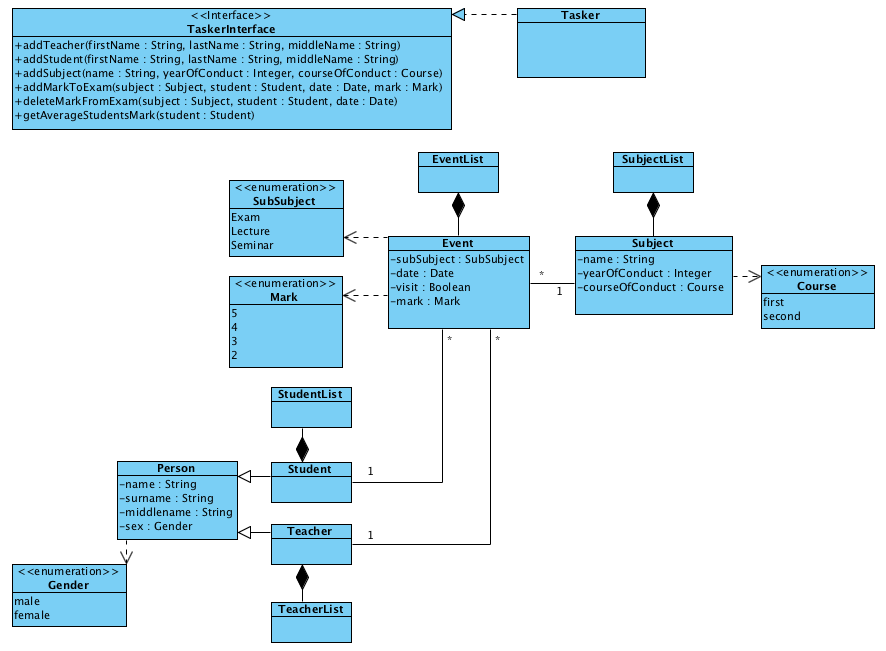
\includegraphics[width=15cm]{img/diag2}
	\end{center}
	\vspace{-5mm}\caption{Диаграмма классов проектирования}
\end{figure}


\newpage
\section{Диаграмма последовательностей}

\begin{figure}[hhh!]
	\begin{center}
		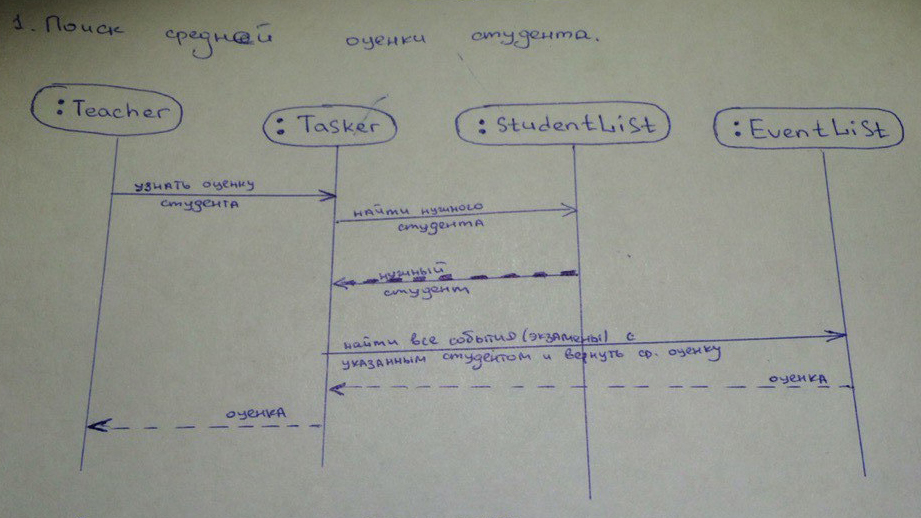
\includegraphics[width=15cm]{img/diagPo1}
	\end{center}
	\vspace{-5mm}\caption{Диаграмма последовательностей (часть 1)}
\end{figure}

\begin{figure}[hhh!]
	\begin{center}
		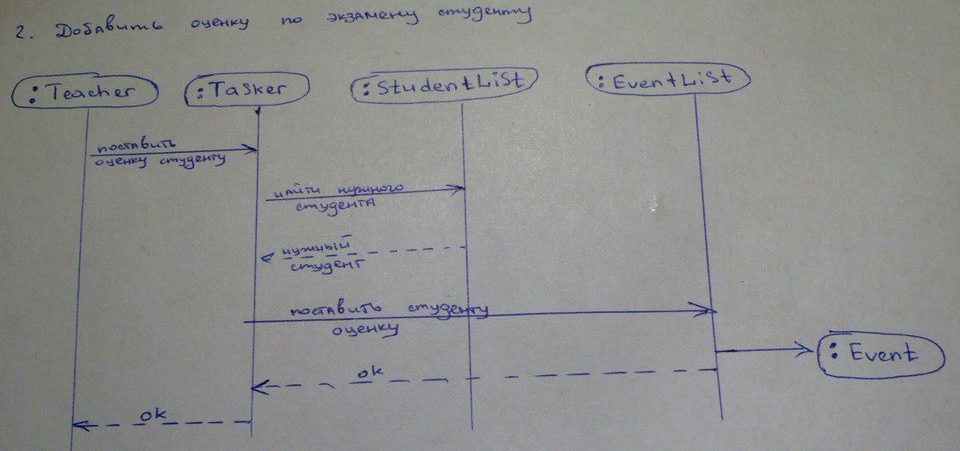
\includegraphics[width=15cm]{img/diagPo2}
	\end{center}
	\vspace{-5mm}\caption{Диаграмма последовательностей (часть 2)}
\end{figure}

\chapter{Выводы}



\end{document}
